\documentclass{article}\usepackage[]{graphicx}\usepackage[]{color}
% maxwidth is the original width if it is less than linewidth
% otherwise use linewidth (to make sure the graphics do not exceed the margin)
\makeatletter
\def\maxwidth{ %
  \ifdim\Gin@nat@width>\linewidth
    \linewidth
  \else
    \Gin@nat@width
  \fi
}
\makeatother

\definecolor{fgcolor}{rgb}{0.345, 0.345, 0.345}
\newcommand{\hlnum}[1]{\textcolor[rgb]{0.686,0.059,0.569}{#1}}%
\newcommand{\hlstr}[1]{\textcolor[rgb]{0.192,0.494,0.8}{#1}}%
\newcommand{\hlcom}[1]{\textcolor[rgb]{0.678,0.584,0.686}{\textit{#1}}}%
\newcommand{\hlopt}[1]{\textcolor[rgb]{0,0,0}{#1}}%
\newcommand{\hlstd}[1]{\textcolor[rgb]{0.345,0.345,0.345}{#1}}%
\newcommand{\hlkwa}[1]{\textcolor[rgb]{0.161,0.373,0.58}{\textbf{#1}}}%
\newcommand{\hlkwb}[1]{\textcolor[rgb]{0.69,0.353,0.396}{#1}}%
\newcommand{\hlkwc}[1]{\textcolor[rgb]{0.333,0.667,0.333}{#1}}%
\newcommand{\hlkwd}[1]{\textcolor[rgb]{0.737,0.353,0.396}{\textbf{#1}}}%
\let\hlipl\hlkwb

\usepackage{framed}
\makeatletter
\newenvironment{kframe}{%
 \def\at@end@of@kframe{}%
 \ifinner\ifhmode%
  \def\at@end@of@kframe{\end{minipage}}%
  \begin{minipage}{\columnwidth}%
 \fi\fi%
 \def\FrameCommand##1{\hskip\@totalleftmargin \hskip-\fboxsep
 \colorbox{shadecolor}{##1}\hskip-\fboxsep
     % There is no \\@totalrightmargin, so:
     \hskip-\linewidth \hskip-\@totalleftmargin \hskip\columnwidth}%
 \MakeFramed {\advance\hsize-\width
   \@totalleftmargin\z@ \linewidth\hsize
   \@setminipage}}%
 {\par\unskip\endMakeFramed%
 \at@end@of@kframe}
\makeatother

\definecolor{shadecolor}{rgb}{.97, .97, .97}
\definecolor{messagecolor}{rgb}{0, 0, 0}
\definecolor{warningcolor}{rgb}{1, 0, 1}
\definecolor{errorcolor}{rgb}{1, 0, 0}
\newenvironment{knitrout}{}{} % an empty environment to be redefined in TeX

\usepackage{alltt}

\title{Seminar 5}
\author{Louisa Boulaziz}
\date{\today}
\IfFileExists{upquote.sty}{\usepackage{upquote}}{}
\begin{document}
\maketitle

\hfill \break I dag skal vi jobbe med det samme datasettet som sist gang ettersom vi kjenner variablene. Det kan være lurt når vi begynner med regresjonsanalyse. Vi begynner med å laste inn pakker og data. Vi skal bruke en ny pakke i dag. Denne må dere ta install.packages("modlr") først, også library som under. 

\begin{knitrout}
\definecolor{shadecolor}{rgb}{0.969, 0.969, 0.969}\color{fgcolor}\begin{kframe}
\begin{alltt}
\hlcom{# Pakker }
\hlkwd{library}\hlstd{(tidyverse)}
\end{alltt}


{\ttfamily\noindent\itshape\color{messagecolor}{\#\# -- Attaching packages --------------------------------------- tidyverse 1.3.0 --}}

{\ttfamily\noindent\itshape\color{messagecolor}{\#\# v ggplot2 3.3.2\ \ \ \  v purrr\ \  0.3.4\\\#\# v tibble\ \ 3.0.6\ \ \ \  v dplyr\ \  1.0.2\\\#\# v tidyr\ \  1.1.2\ \ \ \  v stringr 1.4.0\\\#\# v readr\ \  1.4.0\ \ \ \  v forcats 0.5.0}}

{\ttfamily\noindent\itshape\color{messagecolor}{\#\# -- Conflicts ------------------------------------------ tidyverse\_conflicts() --\\\#\# x dplyr::filter() masks stats::filter()\\\#\# x dplyr::lag()\ \ \ \ masks stats::lag()}}\begin{alltt}
\hlkwd{library}\hlstd{(stargazer)}
\end{alltt}


{\ttfamily\noindent\itshape\color{messagecolor}{\#\# \\\#\# Please cite as:}}

{\ttfamily\noindent\itshape\color{messagecolor}{\#\#\ \ Hlavac, Marek (2018). stargazer: Well-Formatted Regression and Summary Statistics Tables.}}

{\ttfamily\noindent\itshape\color{messagecolor}{\#\#\ \ R package version 5.2.2. https://CRAN.R-project.org/package=stargazer}}\begin{alltt}
\hlkwd{library}\hlstd{(modelr)}

\hlcom{# Laser inn data }
\hlstd{data} \hlkwb{<-} \hlkwd{read.csv}\hlstd{(}\hlstr{"https://raw.githubusercontent.com/louisabo/STV4020A/master/SEMINAR3/internett.csv"}\hlstd{)}
\end{alltt}
\end{kframe}
\end{knitrout}

\hfill \break Jeg bruker read.csv fordi dataene er csv-fil og de er lastet ned direkte fra internett. Når jeg gjør dette trenger jeg i prinsippet ikke å sette et "working directory." 
\hfill \break Vi skal jobbe videre med NA. Se på noen andre koder vi kan bruke for å fiske ut NA. NA som dere husker er missing-verdier og disse må vi identifisere. Koden complete.cases viser hvor mange fullstendige eller ufullstendige rader det er i datasettet. Det vil si at denne koden identifiserer alle rader som har NA på en eller flere variable. Du kan bruke table for å printe dem

\begin{knitrout}
\definecolor{shadecolor}{rgb}{0.969, 0.969, 0.969}\color{fgcolor}\begin{kframe}
\begin{alltt}
\hlkwd{table}\hlstd{(}\hlkwd{complete.cases}\hlstd{(data))} \hlcom{# Viser ufullstendige rader}
\end{alltt}
\begin{verbatim}
## 
## FALSE  TRUE 
##   183  2562
\end{verbatim}
\begin{alltt}
\hlkwd{table}\hlstd{(}\hlkwd{is.na}\hlstd{(data}\hlopt{$}\hlstd{internettbruk))} \hlcom{# Viser antall NA på variabel}
\end{alltt}
\begin{verbatim}
## 
## FALSE  TRUE 
##  2740     5
\end{verbatim}
\begin{alltt}
\hlcom{# Vi kan legge NA i et eget datasett:}

\hlstd{missing_2} \hlkwb{<-} \hlstd{data} \hlopt
  \hlkwd{filter_all}\hlstd{(}\hlkwd{any_vars}\hlstd{(}\hlkwd{is.na}\hlstd{(.)))}
\end{alltt}
\end{kframe}
\end{knitrout}

\hfill \break Vi kan også lage en ny variabel i datasettet som flagger NA-rader -- altså rader eller observasjoner som har NA på en eller flere variable. Dette kan vi gjøre på alle variable, eventuelt bare flagge rader som har NA på en spesifikk variabel. Vi bruker mutate fra tidyverse-pakken til å opprette to nye variabler. 

\begin{knitrout}
\definecolor{shadecolor}{rgb}{0.969, 0.969, 0.969}\color{fgcolor}\begin{kframe}
\begin{alltt}
\hlstd{data} \hlkwb{<-} \hlstd{data} \hlopt
  \hlkwd{mutate}\hlstd{(}\hlkwc{complete} \hlstd{=} \hlkwd{complete.cases}\hlstd{(.),}   \hlcom{# ny var 1}
         \hlkwc{internett_na} \hlstd{=} \hlkwd{is.na}\hlstd{(internettbruk))} \hlcom{# ny var 2}


\hlkwd{table}\hlstd{(data}\hlopt{$}\hlstd{internett_na)}
\end{alltt}
\begin{verbatim}
## 
## FALSE  TRUE 
##  2740     5
\end{verbatim}
\begin{alltt}
\hlkwd{table}\hlstd{(data}\hlopt{$}\hlstd{complete)}
\end{alltt}
\begin{verbatim}
## 
## FALSE  TRUE 
##   183  2562
\end{verbatim}
\end{kframe}
\end{knitrout}

\hifill \break Her fjerner alle NA også jobber vi videre. Merk at jeg også fjerner de nye variablene jeg nettopp opprettet fordi ønsker jeg ikke å ha med meg videre. Du kan bruke select funksjonen etter drop_na() og deretter bare tall for å si til R hvilke variable du velge. Jeg vil velge de første fem, så jeg skriver 1:5. 

\begin{knitrout}
\definecolor{shadecolor}{rgb}{0.969, 0.969, 0.969}\color{fgcolor}\begin{kframe}
\begin{alltt}
\hlstd{data} \hlkwb{<-} \hlstd{data} \hlopt
  \hlkwd{drop_na}\hlstd{()} \hlopt
  \hlkwd{select}\hlstd{(}\hlnum{1}\hlopt{:}\hlnum{5}\hlstd{)}
\end{alltt}
\end{kframe}
\end{knitrout}

\hfill \break Før vi går videre med regresjonsanalyse må vi repetere litt oppretting av nye variable. Dette er veldig viktig å kunne og dere må øve på dette før prøven. Som alltid i R finnes det mye kode som gjør det samme. Jeg skal vise litt forskjellige omkodinger. Først omkoder vi variabelen kjønn. Nå viser den 1 for menn og 2 for kvinner. Jeg vil at den skal vise 0 for menn og 1 for kvinner. 

\begin{knitrout}
\definecolor{shadecolor}{rgb}{0.969, 0.969, 0.969}\color{fgcolor}\begin{kframe}
\begin{alltt}
\hlstd{data}\hlopt{$}\hlstd{kjonn_1} \hlkwb{<-} \hlkwd{ifelse}\hlstd{(data}\hlopt{$}\hlstd{kjonn} \hlopt{==} \hlnum{1}\hlstd{,} \hlnum{0}\hlstd{,} \hlnum{1}\hlstd{)}

\hlcom{# Sjekker at det blir riktig }
\hlkwd{table}\hlstd{(data}\hlopt{$}\hlstd{kjonn_1)}
\end{alltt}
\begin{verbatim}
## 
##    0    1 
## 1211 1351
\end{verbatim}
\end{kframe}
\end{knitrout}

\hfill \break Vi skal foreta en litt vanskeligere omkoding hvor vi koder om utdanning til en variabel som måler utdanning i kategori istedet for kontiuerlig. Vi skal opprette fire kategorier: 

\begin{itemize}
\item Alle som har antall år med utdanning 0-10 = lav
\item Alle som har antall år med utdanning 11-20 = mellom
\item Alle som har antall år med utdanning 21-30 = hoy
\item Alle som har antall år med utdanning 31-37 = veldig hoy
\end{itemize}

\hfill \break Mutate er bra for store og flere omkodinger samtidig. Jeg vil bare legge til at denne koden er ikke noe jeg forventer dere må huske, men det er viktig at dere prøver å se om dere forstår logikken og syntaksen. Det er ekstremt viktig å prøve å forstå hva koden gjør, mer enn å huske den utenatt. 
\begin{knitrout}
\definecolor{shadecolor}{rgb}{0.969, 0.969, 0.969}\color{fgcolor}\begin{kframe}
\begin{alltt}
\hlstd{data} \hlkwb{<-} \hlstd{data} \hlopt
  \hlkwd{mutate}\hlstd{(}\hlkwc{utdanning_1} \hlstd{=} \hlkwd{case_when}\hlstd{(utdanning} \hlopt{>=}\hlnum{0} \hlopt{&}
                                   \hlstd{utdanning} \hlopt{<=} \hlnum{10} \hlopt{~} \hlstr{"lav"}\hlstd{,}
                                 \hlstd{utdanning} \hlopt{>=}\hlnum{11} \hlopt{&}
                                   \hlstd{utdanning} \hlopt{<=} \hlnum{20}
                                 \hlopt{~}\hlstr{"middels"}
                                   \hlstd{, utdanning} \hlopt{>=} \hlnum{21} \hlopt{&}
                                   \hlstd{utdanning} \hlopt{<=} \hlnum{30} \hlopt{~} \hlstr{"hoy"}\hlstd{,}
                                 \hlstd{utdanning} \hlopt{>=}\hlnum{30} \hlopt{&} \hlstd{utdanning}
                                 \hlopt{<=} \hlnum{37} \hlopt{~} \hlstr{"veldig hoy"}\hlstd{))}

\hlcom{# Ser at det blir riktig: }
\hlkwd{table}\hlstd{(data}\hlopt{$}\hlstd{utdanning_1)}
\end{alltt}
\begin{verbatim}
## 
##        hoy        lav    middels veldig hoy 
##         37       1034       1490          1
\end{verbatim}
\begin{alltt}
\hlkwd{table}\hlstd{(data}\hlopt{$}\hlstd{utdanning_1, data}\hlopt{$}\hlstd{utdanning)}
\end{alltt}
\begin{verbatim}
##             
##                0   1   2   3   4   5   6   7   8   9  10  11  12  13  14  15
##   hoy          0   0   0   0   0   0   0   0   0   0   0   0   0   0   0   0
##   lav          2   3  11  33  12 227  31  25 490  67 133   0   0   0   0   0
##   middels      0   0   0   0   0   0   0   0   0   0   0 131 136 595 126  93
##   veldig hoy   0   0   0   0   0   0   0   0   0   0   0   0   0   0   0   0
##             
##               16  17  18  19  20  21  22  23  24  25  26  27  30  37
##   hoy          0   0   0   0   0  10   8  10   2   2   1   1   3   0
##   lav          0   0   0   0   0   0   0   0   0   0   0   0   0   0
##   middels    110  57 135  55  52   0   0   0   0   0   0   0   0   0
##   veldig hoy   0   0   0   0   0   0   0   0   0   0   0   0   0   1
\end{verbatim}
\end{kframe}
\end{knitrout}

\hfill \break Som om denne koden ikke var nok, så skal vi omkode denne variabelen til å lage en dikotom utdanningsvariabel av den vi har laget med fire nivåer. Nå bruker jeg bare ifelse og ikke mutate for å vise. Disse kodene blir litt lange så det gjelder å holde tunga rett i munnen. Her koder jeg om alle som har lav og middels utdanning til 0 og alle som har høy og veldig høy utdanning til 1. 

\begin{knitrout}
\definecolor{shadecolor}{rgb}{0.969, 0.969, 0.969}\color{fgcolor}\begin{kframe}
\begin{alltt}
\hlstd{data}\hlopt{$}\hlstd{utdanning_2} \hlkwb{<-} \hlkwd{ifelse}\hlstd{(data}\hlopt{$}\hlstd{utdanning_1} \hlopt{==} \hlstr{"lav"}\hlstd{,} \hlnum{0}\hlstd{,}
                           \hlkwd{ifelse}\hlstd{(data}\hlopt{$}\hlstd{utdanning_1} \hlopt{==} \hlstr{"middels"}\hlstd{,} \hlnum{0}\hlstd{,}
                                  \hlkwd{ifelse}\hlstd{(data}\hlopt{$}\hlstd{utdanning_1} \hlopt{==} \hlstr{"hoy"}\hlstd{,} \hlnum{1}\hlstd{,}
                                         \hlkwd{ifelse}\hlstd{(data}\hlopt{$}\hlstd{utdanning_1} \hlopt{==} \hlstr{"veldig hoy"}\hlstd{,} \hlnum{1}\hlstd{,}
                                                \hlkwd{ifelse}\hlstd{(data}\hlopt{$}\hlstd{utdanning_1)))))}

\hlcom{# Ser at det blir riktig }

\hlkwd{table}\hlstd{(data}\hlopt{$}\hlstd{utdanning_2)}
\end{alltt}
\begin{verbatim}
## 
##    0    1 
## 2524   38
\end{verbatim}
\begin{alltt}
\hlkwd{table}\hlstd{(data}\hlopt{$}\hlstd{utdanning_1, data}\hlopt{$}\hlstd{utdanning_2)}
\end{alltt}
\begin{verbatim}
##             
##                 0    1
##   hoy           0   37
##   lav        1034    0
##   middels    1490    0
##   veldig hoy    0    1
\end{verbatim}
\begin{alltt}
\hlcom{# Vi kan plotte variablene dataene våre: }

\hlkwd{ggplot}\hlstd{(data,} \hlkwd{aes}\hlstd{(utdanning_1))} \hlopt{+}
  \hlkwd{geom_bar}\hlstd{()}
\end{alltt}
\end{kframe}
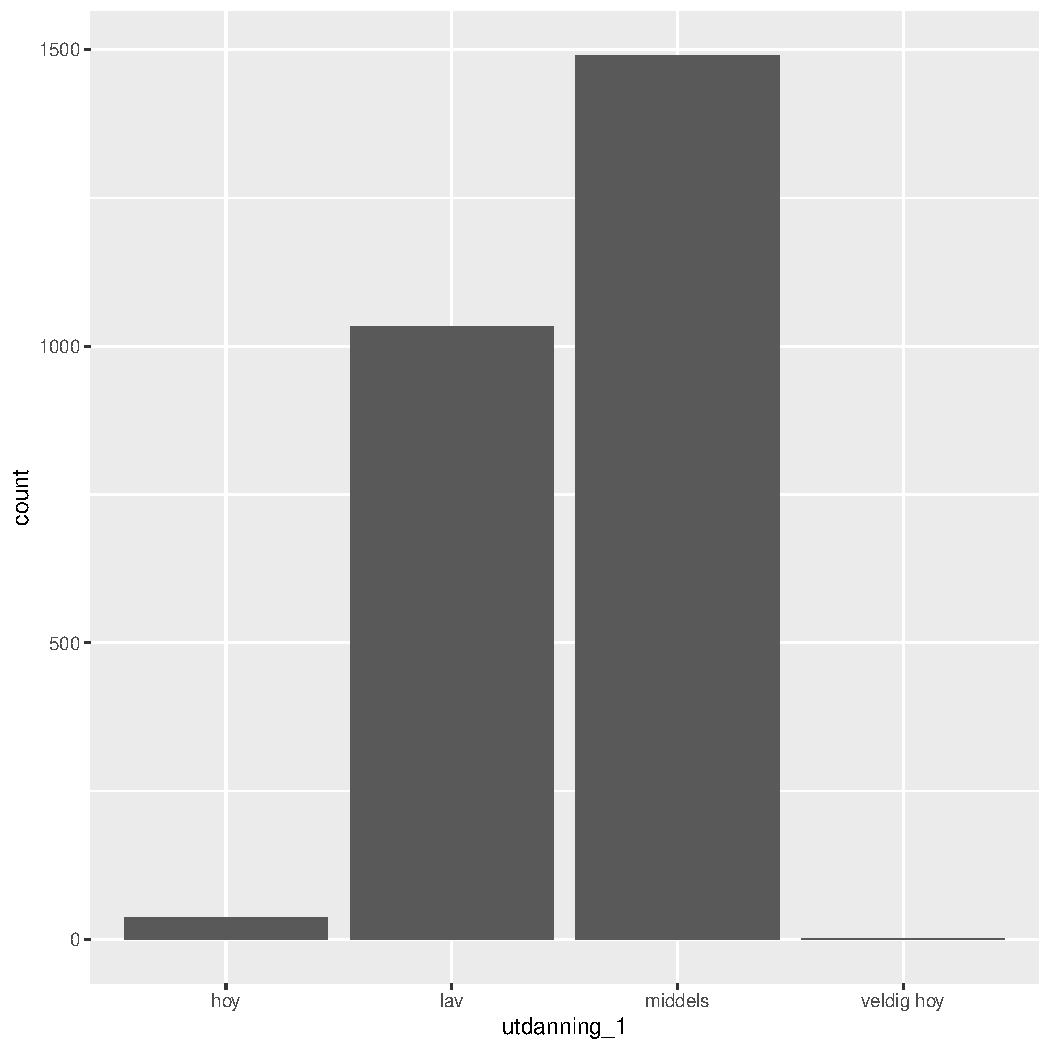
\includegraphics[width=\maxwidth]{figure/lager_mer_utdanning-1} 
\begin{kframe}\begin{alltt}
\hlkwd{ggplot}\hlstd{(data,} \hlkwd{aes}\hlstd{(utdanning_2))} \hlopt{+}
  \hlkwd{geom_bar}\hlstd{()} \hlopt{+}
  \hlkwd{scale_x_discrete}\hlstd{()} \hlopt{+}
  \hlkwd{xlab}\hlstd{(}\hlstr{"Utdanning"}\hlstd{)} \hlopt{+}
  \hlkwd{ylab}\hlstd{(}\hlstr{"frekvens"}\hlstd{)}
\end{alltt}
\end{kframe}
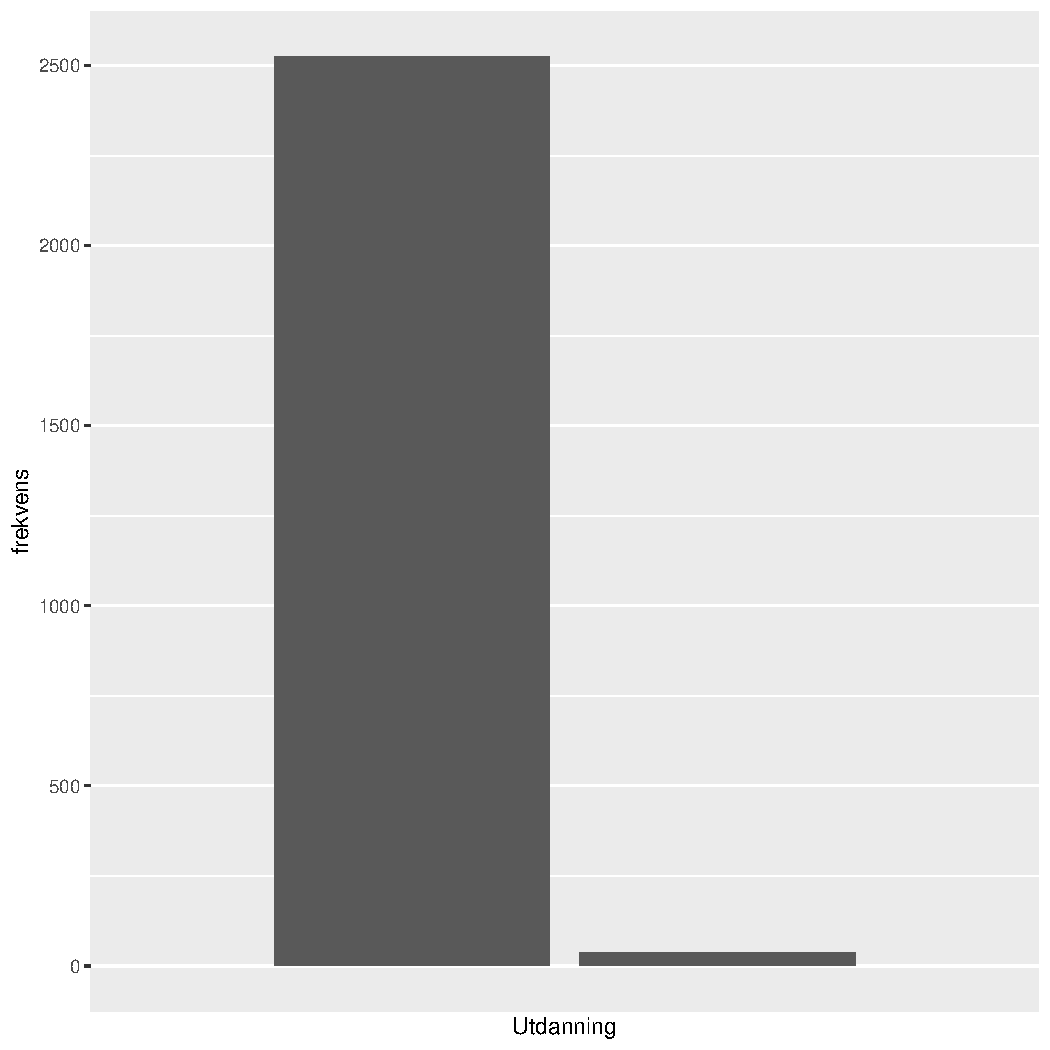
\includegraphics[width=\maxwidth]{figure/lager_mer_utdanning-2} 

\end{knitrout}


\hfill \break Før vi går videre til regresjon så sjekker vi klasse og fjerner de variablene vi ikke vil ha i datasettet. Jeg bruker igjen select og subsetter. Deretter koder jeg om den nye kjonnvariabelen til å bare hete kjonn.

\begin{knitrout}
\definecolor{shadecolor}{rgb}{0.969, 0.969, 0.969}\color{fgcolor}\begin{kframe}
\begin{alltt}
\hlkwd{str}\hlstd{(data)}
\end{alltt}
\begin{verbatim}
## 'data.frame':	2562 obs. of  8 variables:
##  $ internettbruk: int  5 5 1 1 5 1 5 1 4 1 ...
##  $ kjonn        : int  2 1 2 2 2 1 2 2 1 2 ...
##  $ alder        : int  67 45 73 86 53 77 35 66 52 86 ...
##  $ utdanning    : int  18 11 8 3 17 18 18 16 10 3 ...
##  $ tillit       : int  8 6 0 6 6 0 3 6 6 7 ...
##  $ kjonn_1      : num  1 0 1 1 1 0 1 1 0 1 ...
##  $ utdanning_1  : chr  "middels" "middels" "lav" "lav" ...
##  $ utdanning_2  : num  0 0 0 0 0 0 0 0 0 0 ...
\end{verbatim}
\begin{alltt}
\hlcom{# Vi subsetter og tar med de variablene vi er interessert i }

\hlstd{df} \hlkwb{<-} \hlstd{data} \hlopt
  \hlkwd{select}\hlstd{(internettbruk, alder, utdanning, tillit, kjonn_1)}

\hlstd{df} \hlkwb{<-} \hlstd{df} \hlopt
  \hlkwd{rename}\hlstd{(}\hlkwc{kjonn} \hlstd{= kjonn_1)}
\end{alltt}
\end{kframe}
\end{knitrout}


\hfill \break \textbf{REGRESJON MED NUMERISK UAVHENGIG VARIABEL}
For å kjøre en lineær regresjon i R så bruker vi funksjonen lm(). lm() har følgende syntaks:
\begin{knitrout}
\definecolor{shadecolor}{rgb}{0.969, 0.969, 0.969}\color{fgcolor}\begin{kframe}
\begin{alltt}
\hlkwd{lm}\hlstd{(avhengig_variabel} \hlopt{~} \hlstd{uavhengig_variabel,} \hlkwc{data} \hlstd{= mitt_datasett)}
\end{alltt}
\end{kframe}
\end{knitrout}
\hfill \break Dersom datasettet ditt har manglende informasjon (missing/NA) så må du legge til et element som sier hvor- dan regresjonen skal forholde seg til dette. Ved å legge til na.action = "na.exclude" i lm()så beholder R informasjon om hvilke observasjoner som mangler data. 

\hfill \break Vi skal nå kjøre en regresjon med internettbruk og alder. Vi har fjernet NA så vi trenger ikke na.action-argumentet. Resulatene fra regresjonen vi får ved hjelp av summary() og stargazer() er veldig nyttig. Vi får vite koeffisientene, standardfeilene og informasjon vi kan bruke til å evaluere modellen vår. I seminar skal vi bruke en del tid på å tolke disse tabellene.

\begin{knitrout}
\definecolor{shadecolor}{rgb}{0.969, 0.969, 0.969}\color{fgcolor}\begin{kframe}
\begin{alltt}
\hlstd{mod} \hlkwb{<-} \hlkwd{lm}\hlstd{(internettbruk} \hlopt{~} \hlstd{alder,} \hlkwc{data} \hlstd{= df)}
\hlkwd{summary}\hlstd{(mod)}
\end{alltt}
\begin{verbatim}
## 
## Call:
## lm(formula = internettbruk ~ alder, data = df)
## 
## Residuals:
##     Min      1Q  Median      3Q     Max 
## -4.4400 -0.9129 -0.0071  0.9378  3.1973 
## 
## Coefficients:
##              Estimate Std. Error t value Pr(>|t|)    
## (Intercept)  6.487113   0.070921   91.47   <2e-16 ***
## alder       -0.055111   0.001292  -42.64   <2e-16 ***
## ---
## Signif. codes:  0 '***' 0.001 '**' 0.01 '*' 0.05 '.' 0.1 ' ' 1
## 
## Residual standard error: 1.255 on 2560 degrees of freedom
## Multiple R-squared:  0.4153,	Adjusted R-squared:  0.4151 
## F-statistic:  1818 on 1 and 2560 DF,  p-value: < 2.2e-16
\end{verbatim}
\begin{alltt}
\hlcom{# For mer oversikt bruk stargazer }

\hlkwd{stargazer}\hlstd{(mod,} \hlkwc{type} \hlstd{=} \hlstr{"text"}\hlstd{)}
\end{alltt}
\begin{verbatim}
## 
## ===============================================
##                         Dependent variable:    
##                     ---------------------------
##                            internettbruk       
## -----------------------------------------------
## alder                        -0.055***         
##                               (0.001)          
##                                                
## Constant                     6.487***          
##                               (0.071)          
##                                                
## -----------------------------------------------
## Observations                   2,562           
## R2                             0.415           
## Adjusted R2                    0.415           
## Residual Std. Error      1.255 (df = 2560)     
## F Statistic         1,818.322*** (df = 1; 2560)
## ===============================================
## Note:               *p<0.1; **p<0.05; ***p<0.01
\end{verbatim}
\end{kframe}
\end{knitrout}

\hfill \break Vi må tolke resultatene vi får ut. Da kan det være viktig å først bare tenke på retning og signfikans. Deretter bør vi gå tilbake å tenke på hva er analyseenheten/observasjonsenheten og hvilket målenivå er variablene jeg analyserer? Vi må tolke både konstantledd og estimatet. 

\hfill \break Ved hjelp av stargazer så kan vi også lagre tabeller lokalt på PC-en som vi kan bruke i word-dokumenter og liknende. Da endrer vi på type argumentet og legger til et out argument. out argumentet forteller i hvilken mappe du vil lagre filen samt hva filen skal hete. Da får du en .htm-fil som ser omtrent ut som i eksempelet under. Den kan du høyreklikke på og velge åpne i word dersom du skal ha tabellen inn i en oppgave eller liknende. Dette viste jeg sist gang. 

\hfill \break Jeg synes ofte det vanskelig å tolke tallene, derfor er det så viktig å plotte tallene man får ut. Akkurat slik vi gjore sist gang. Det som er fint nå er at med modellen vi har laget har vi en OLS linje som vi kan plotte. Det er nå vi skal bruke modelr-pakken. Denne står det mye mer om i kapittel 23 i R for data Science som er lenket til på Canvas. I plottet under skal vi plotte prediksjonene våre -- altså de predikerte verdiene som model vår estimerer på bakgrunn av observasjonene i dataene. Vi lagrer prediksjonene i et eget objekt som jeg kaller prediksjoner. 

\begin{knitrout}
\definecolor{shadecolor}{rgb}{0.969, 0.969, 0.969}\color{fgcolor}\begin{kframe}
\begin{alltt}
\hlstd{prediksjoner} \hlkwb{<-} \hlstd{df} \hlopt
  \hlkwd{add_predictions}\hlstd{(mod,} \hlstr{"internettbruk"}\hlstd{)}

\hlcom{# add_pred tar to argumenter: model og avhengig var}

\hlcom{# Ggplot }
\hlkwd{ggplot}\hlstd{(df,} \hlkwd{aes}\hlstd{(alder, internettbruk))} \hlopt{+}
  \hlkwd{geom_smooth}\hlstd{(}\hlkwc{data} \hlstd{= prediksjoner,} \hlkwc{colour} \hlstd{=} \hlstr{"red"}\hlstd{,}
            \hlkwc{size} \hlstd{=} \hlnum{1}\hlstd{)} \hlopt{+}
  \hlkwd{ggtitle}\hlstd{(}\hlstr{"Linær sammenheng mellom alder og internettbruk"}\hlstd{)}
\end{alltt}


{\ttfamily\noindent\itshape\color{messagecolor}{\#\# `geom\_smooth()` using method = 'gam' and formula 'y \textasciitilde{} s(x, bs = "{}cs"{})'}}\end{kframe}
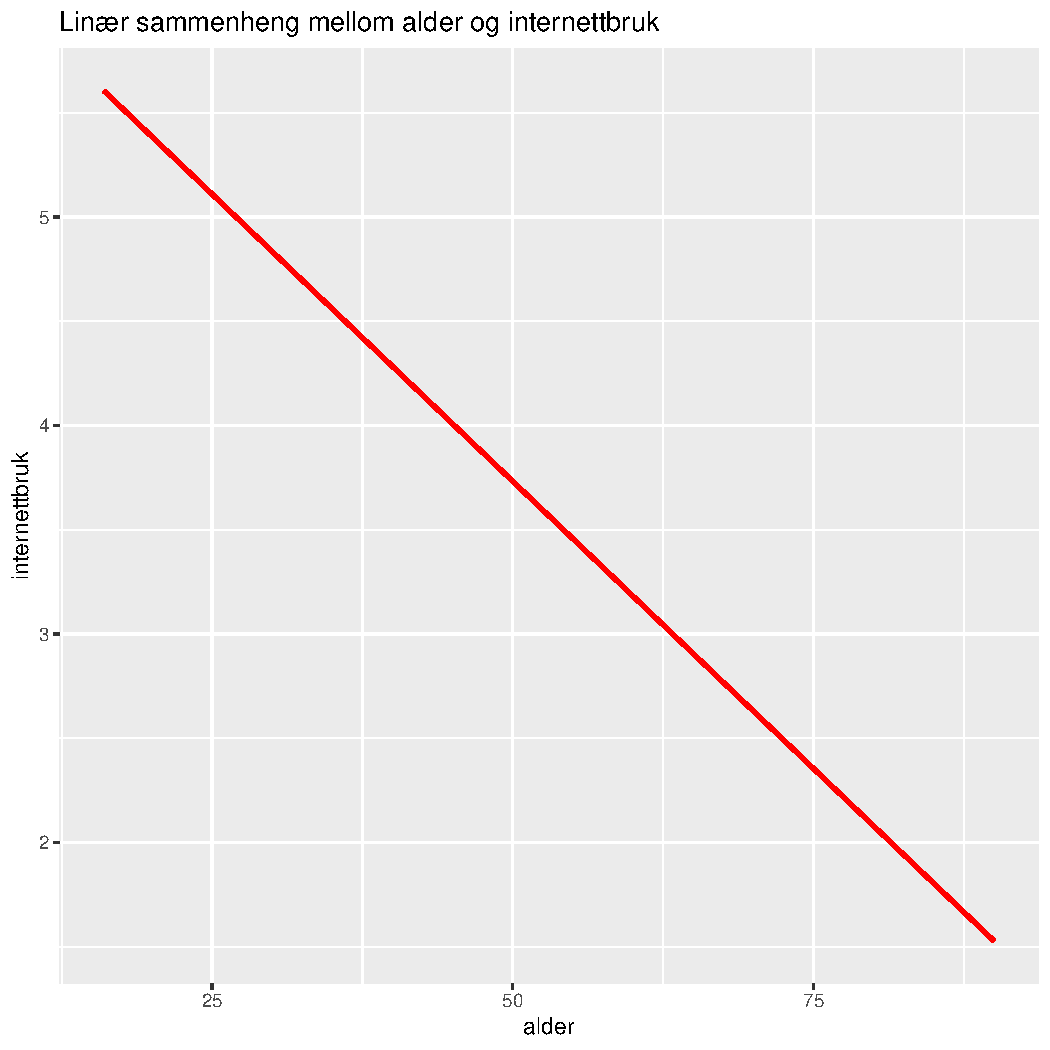
\includegraphics[width=\maxwidth]{figure/prediksjonsplott-1} 
\begin{kframe}\begin{alltt}
\hlcom{# Legg merge til at linjen kommer fra prediksjons-dataene vi nettopp lagde. }
\end{alltt}
\end{kframe}
\end{knitrout}

\hfill \break Vi kan se konfidensintervallet til estimatet og konstantleddet med følgende kode. 

\begin{knitrout}
\definecolor{shadecolor}{rgb}{0.969, 0.969, 0.969}\color{fgcolor}\begin{kframe}
\begin{alltt}
\hlkwd{confint}\hlstd{(mod)}
\end{alltt}
\begin{verbatim}
##                  2.5 %      97.5 %
## (Intercept)  6.3480442  6.62618271
## alder       -0.0576456 -0.05257699
\end{verbatim}
\end{kframe}
\end{knitrout}


\hfill \break \textbf{Regresjon med dikotom uavhengig variabel}

\hfill \break Vi skal nå kjøre regresjon med tillit og kjønn. Dette gjør vi mest for å øve oss på å tolke resultater. Tenk på målenivå de to ulike variablene. 

\begin{knitrout}
\definecolor{shadecolor}{rgb}{0.969, 0.969, 0.969}\color{fgcolor}\begin{kframe}
\begin{alltt}
\hlstd{mod1} \hlkwb{<-} \hlkwd{lm}\hlstd{(tillit} \hlopt{~} \hlstd{kjonn,} \hlkwc{data} \hlstd{= df)}
\hlkwd{summary}\hlstd{(mod1)}
\end{alltt}
\begin{verbatim}
## 
## Call:
## lm(formula = tillit ~ kjonn, data = df)
## 
## Residuals:
##     Min      1Q  Median      3Q     Max 
## -4.3666 -2.1710  0.6334  1.8290  5.8290 
## 
## Coefficients:
##             Estimate Std. Error t value Pr(>|t|)    
## (Intercept)  4.36664    0.07215  60.521   <2e-16 ***
## kjonn       -0.19565    0.09936  -1.969    0.049 *  
## ---
## Signif. codes:  0 '***' 0.001 '**' 0.01 '*' 0.05 '.' 0.1 ' ' 1
## 
## Residual standard error: 2.511 on 2560 degrees of freedom
## Multiple R-squared:  0.001512,	Adjusted R-squared:  0.001122 
## F-statistic: 3.878 on 1 and 2560 DF,  p-value: 0.04904
\end{verbatim}
\begin{alltt}
\hlcom{# Vi kan også printe disse resultatene med }
\hlcom{# stargazer }

\hlkwd{stargazer}\hlstd{(mod1,} \hlkwc{type} \hlstd{=} \hlstr{"text"}\hlstd{)}
\end{alltt}
\begin{verbatim}
## 
## ===============================================
##                         Dependent variable:    
##                     ---------------------------
##                               tillit           
## -----------------------------------------------
## kjonn                        -0.196**          
##                               (0.099)          
##                                                
## Constant                     4.367***          
##                               (0.072)          
##                                                
## -----------------------------------------------
## Observations                   2,562           
## R2                             0.002           
## Adjusted R2                    0.001           
## Residual Std. Error      2.511 (df = 2560)     
## F Statistic           3.878** (df = 1; 2560)   
## ===============================================
## Note:               *p<0.1; **p<0.05; ***p<0.01
\end{verbatim}
\end{kframe}
\end{knitrout}

\hfill \break Vi plotter også resultatene fra denne regresjonen. 

\begin{knitrout}
\definecolor{shadecolor}{rgb}{0.969, 0.969, 0.969}\color{fgcolor}\begin{kframe}
\begin{alltt}
\hlstd{prediksjoner1} \hlkwb{<-} \hlstd{df} \hlopt
  \hlkwd{add_predictions}\hlstd{(mod1,} \hlstr{"tillit"}\hlstd{)}


\hlcom{# Det ser litt rart ut }
\hlkwd{ggplot}\hlstd{(df,} \hlkwd{aes}\hlstd{(kjonn, tillit))} \hlopt{+}
  \hlkwd{geom_line}\hlstd{(}\hlkwc{data} \hlstd{= prediksjoner1)}
\end{alltt}
\end{kframe}
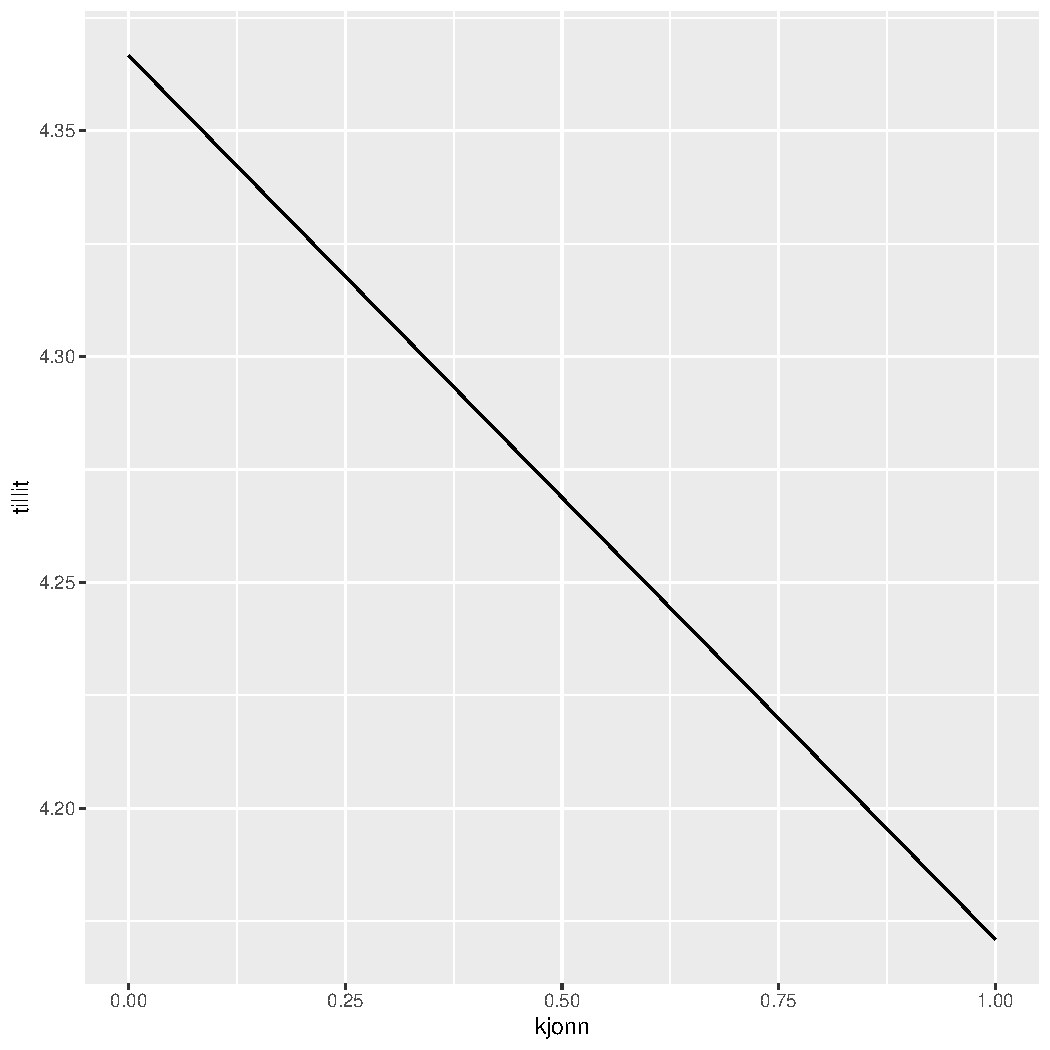
\includegraphics[width=\maxwidth]{figure/resultater_mod2-1} 
\begin{kframe}\begin{alltt}
\hlcom{# Vi kan legge på argumenter: }
\hlkwd{ggplot}\hlstd{(df,} \hlkwd{aes}\hlstd{(kjonn, tillit))} \hlopt{+}
  \hlkwd{geom_line}\hlstd{(}\hlkwc{data} \hlstd{= prediksjoner1)} \hlopt{+}
  \hlkwd{scale_x_discrete}\hlstd{()} \hlopt{+}
  \hlkwd{ggtitle}\hlstd{(}\hlstr{"Smh mellom tillit og kjonn er negativ"}\hlstd{)} \hlopt{+}
  \hlkwd{xlab}\hlstd{(}\hlstr{"Viser smh for kvinner, mann er ref"}\hlstd{)}
\end{alltt}
\end{kframe}
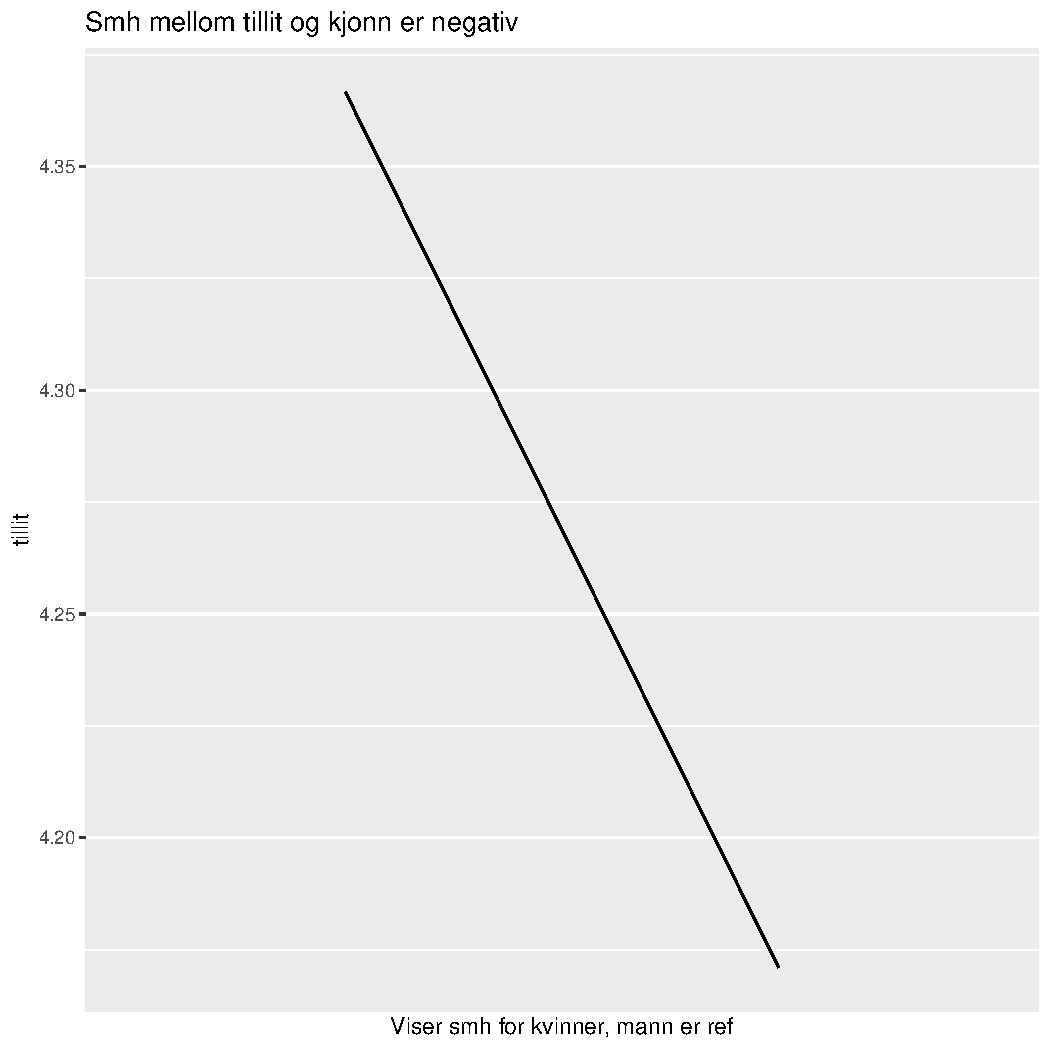
\includegraphics[width=\maxwidth]{figure/resultater_mod2-2} 

\end{knitrout}
\end{document}
